\begin{table*}
\centering
\resizebox{0.8\textwidth}{!}{
\begin{tabular}{@{}m{2cm}@{ }m{3cm}@{ }m{3cm}@{ }m{3cm}@{ }m{3cm}@{ }m{3cm}@{}}
% \toprule
& Llama-3.1-8B & Llama-3.1-70B & Command-R & Jamba-1.5-Mini \\
\midrule
SummHay &
\centering
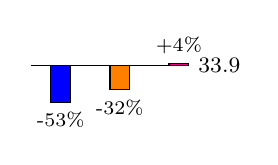
\begin{tikzpicture}[scale=0.5]
\draw (0,2) -- (4,2) node[right, font=\footnotesize] {33.9};
\draw[fill=blue] (0.5,2) rectangle (1,1.06);
\node[below, font=\scriptsize] at (0.75,1.06) {-53\%};
\draw[fill=orange] (2,2) rectangle (2.5,1.37);
\node[below, font=\scriptsize] at (2.25,1.37) {-32\%};
\draw[fill=magenta] (3.5,2) rectangle (4,2.04);
\node[above, font=\scriptsize] at (3.75,2.04) {+4\%};
\end{tikzpicture} &
\centering
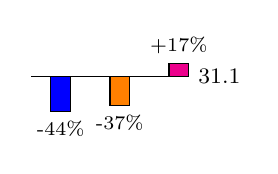
\begin{tikzpicture}[scale=0.5]
\draw (0,2) -- (4,2) node[right, font=\footnotesize] {31.1};
\draw[fill=blue] (0.5,2) rectangle (1,1.11);
\node[below, font=\scriptsize] at (0.75,1.11) {-44\%};
\draw[fill=orange] (2,2) rectangle (2.5,1.27);
\node[below, font=\scriptsize] at (2.25,1.27) {-37\%};
\draw[fill=magenta] (3.5,2) rectangle (4,2.33);
\node[above, font=\scriptsize] at (3.75,2.33) {+17\%};
\end{tikzpicture} &
\centering
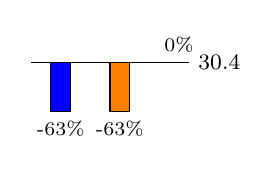
\begin{tikzpicture}[scale=0.5]
\draw (0,2) -- (4,2) node[right, font=\footnotesize] {30.4};
\draw[fill=blue] (0.5,2) rectangle (1,0.75);
\node[below, font=\scriptsize] at (0.75,0.75) {-63\%};
\draw[fill=orange] (2,2) rectangle (2.5,0.75);
\node[below, font=\scriptsize] at (2.25,0.75) {-63\%};
\draw[fill=magenta] (3.5,2) rectangle (4,2);
\node[above, font=\scriptsize] at (3.75,2) {0\%};
\end{tikzpicture} &
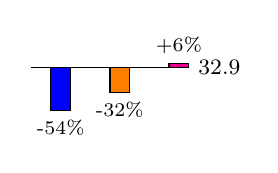
\begin{tikzpicture}[scale=0.5]
\draw (0,2) -- (4,2) node[right, font=\footnotesize] {32.9};
\draw[fill=blue] (0.5,2) rectangle (1,0.92);
\node[below, font=\scriptsize] at (0.75,0.92) {-54\%};
\draw[fill=orange] (2,2) rectangle (2.5,1.37);
\node[below, font=\scriptsize] at (2.25,1.37) {-32\%};
\draw[fill=magenta] (3.5,2) rectangle (4,2.11);
\node[above, font=\scriptsize] at (3.75,2.11) {+6\%};
\end{tikzpicture} \\
SummHay (oracle) &
\centering
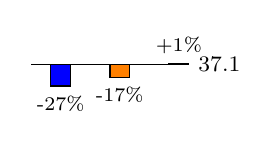
\begin{tikzpicture}[scale=0.5]
\draw (0,2) -- (4,2) node[right, font=\footnotesize] {37.1};
\draw[fill=blue] (0.5,2) rectangle (1,1.45);
\node[below, font=\scriptsize] at (0.75,1.45) {-27\%};
\draw[fill=orange] (2,2) rectangle (2.5,1.67);
\node[below, font=\scriptsize] at (2.25,1.67) {-17\%};
\draw[fill=magenta] (3.5,2) rectangle (4,2.02);
\node[above, font=\scriptsize] at (3.75,2.02) {+1\%};
\end{tikzpicture} &
\centering
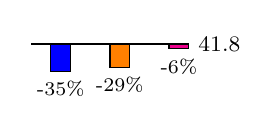
\begin{tikzpicture}[scale=0.5]
\draw (0,2) -- (4,2) node[right, font=\footnotesize] {41.8};
\draw[fill=blue] (0.5,2) rectangle (1,1.30);
\node[below, font=\scriptsize] at (0.75,1.30) {-35\%};
\draw[fill=orange] (2,2) rectangle (2.5,1.41);
\node[below, font=\scriptsize] at (2.25,1.41) {-29\%};
\draw[fill=magenta] (3.5,2) rectangle (4,1.88);
\node[below, font=\scriptsize] at (3.75,1.88) {-6\%};
\end{tikzpicture} &
\centering
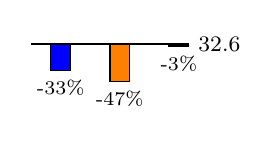
\begin{tikzpicture}[scale=0.5]
\draw (0,2) -- (4,2) node[right, font=\footnotesize] {32.6};
\draw[fill=blue] (0.5,2) rectangle (1,1.33);
\node[below, font=\scriptsize] at (0.75,1.33) {-33\%};
\draw[fill=orange] (2,2) rectangle (2.5,1.05);
\node[below, font=\scriptsize] at (2.25,1.05) {-47\%};
\draw[fill=magenta] (3.5,2) rectangle (4,1.95);
\node[below, font=\scriptsize] at (3.75,1.95) {-3\%};
\end{tikzpicture} &
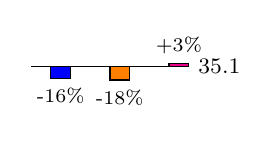
\begin{tikzpicture}[scale=0.5]
\draw (0,2) -- (4,2) node[right, font=\footnotesize] {35.1};
\draw[fill=blue] (0.5,2) rectangle (1,1.69);
\node[below, font=\scriptsize] at (0.75,1.69) {-16\%};
\draw[fill=orange] (2,2) rectangle (2.5,1.65);
\node[below, font=\scriptsize] at (2.25,1.65) {-18\%};
\draw[fill=magenta] (3.5,2) rectangle (4,2.07);
\node[above, font=\scriptsize] at (3.75,2.07) {+3\%};
\end{tikzpicture} \\
Background &
\centering
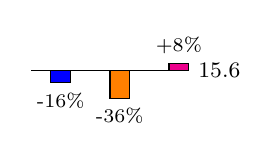
\begin{tikzpicture}[scale=0.5]
\draw (0,2) -- (4,2) node[right, font=\footnotesize] {15.6};
\draw[fill=blue] (0.5,2) rectangle (1,1.68);
\node[below, font=\scriptsize] at (0.75,1.68) {-16\%};
\draw[fill=orange] (2,2) rectangle (2.5,1.28);
\node[below, font=\scriptsize] at (2.25,1.28) {-36\%};
\draw[fill=magenta] (3.5,2) rectangle (4,2.17);
\node[above, font=\scriptsize] at (3.75,2.17) {+8\%};
\end{tikzpicture} &
\centering
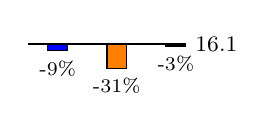
\begin{tikzpicture}[scale=0.5]
\draw (0,2) -- (4,2) node[right, font=\footnotesize] {16.1};
\draw[fill=blue] (0.5,2) rectangle (1,1.83);
\node[below, font=\scriptsize] at (0.75,1.83) {-9\%};
\draw[fill=orange] (2,2) rectangle (2.5,1.38);
\node[below, font=\scriptsize] at (2.25,1.38) {-31\%};
\draw[fill=magenta] (3.5,2) rectangle (4,1.95);
\node[below, font=\scriptsize] at (3.75,1.95) {-3\%};
\end{tikzpicture} &
\centering
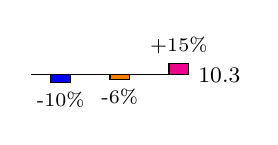
\begin{tikzpicture}[scale=0.5]
\draw (0,2) -- (4,2) node[right, font=\footnotesize] {10.3};
\draw[fill=blue] (0.5,2) rectangle (1,1.81);
\node[below, font=\scriptsize] at (0.75,1.81) {-10\%};
\draw[fill=orange] (2,2) rectangle (2.5,1.88);
\node[below, font=\scriptsize] at (2.25,1.88) {-6\%};
\draw[fill=magenta] (3.5,2) rectangle (4,2.29);
\node[above, font=\scriptsize] at (3.75,2.29) {+15\%};
\end{tikzpicture} &
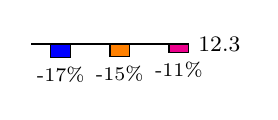
\begin{tikzpicture}[scale=0.5]
\draw (0,2) -- (4,2) node[right, font=\footnotesize] {12.3};
\draw[fill=blue] (0.5,2) rectangle (1,1.66);
\node[below, font=\scriptsize] at (0.75,1.66) {-17\%};
\draw[fill=orange] (2,2) rectangle (2.5,1.69);
\node[below, font=\scriptsize] at (2.25,1.69) {-15\%};
\draw[fill=magenta] (3.5,2) rectangle (4,1.79);
\node[below, font=\scriptsize] at (3.75,1.79) {-11\%};
\end{tikzpicture} \\
WCEP &
\centering
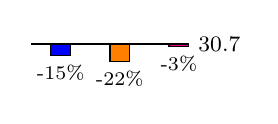
\begin{tikzpicture}[scale=0.5]
\draw (0,2) -- (4,2) node[right, font=\footnotesize] {30.7};
\draw[fill=blue] (0.5,2) rectangle (1,1.71);
\node[below, font=\scriptsize] at (0.75,1.71) {-15\%};
\draw[fill=orange] (2,2) rectangle (2.5,1.56);
\node[below, font=\scriptsize] at (2.25,1.56) {-22\%};
\draw[fill=magenta] (3.5,2) rectangle (4,1.94);
\node[below, font=\scriptsize] at (3.75,1.94) {-3\%};
\end{tikzpicture} &
\centering
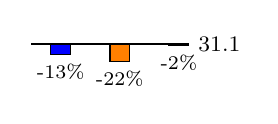
\begin{tikzpicture}[scale=0.5]
\draw (0,2) -- (4,2) node[right, font=\footnotesize] {31.1};
\draw[fill=blue] (0.5,2) rectangle (1,1.74);
\node[below, font=\scriptsize] at (0.75,1.74) {-13\%};
\draw[fill=orange] (2,2) rectangle (2.5,1.56);
\node[below, font=\scriptsize] at (2.25,1.56) {-22\%};
\draw[fill=magenta] (3.5,2) rectangle (4,1.96);
\node[below, font=\scriptsize] at (3.75,1.96) {-2\%};
\end{tikzpicture} &
\centering
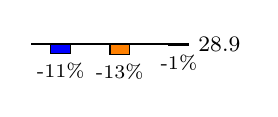
\begin{tikzpicture}[scale=0.5]
\draw (0,2) -- (4,2) node[right, font=\footnotesize] {28.9};
\draw[fill=blue] (0.5,2) rectangle (1,1.77);
\node[below, font=\scriptsize] at (0.75,1.77) {-11\%};
\draw[fill=orange] (2,2) rectangle (2.5,1.74);
\node[below, font=\scriptsize] at (2.25,1.74) {-13\%};
\draw[fill=magenta] (3.5,2) rectangle (4,1.97);
\node[below, font=\scriptsize] at (3.75,1.97) {-1\%};
\end{tikzpicture} &
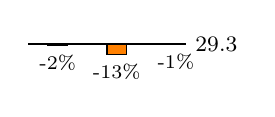
\begin{tikzpicture}[scale=0.5]
\draw (0,2) -- (4,2) node[right, font=\footnotesize] {29.3};
\draw[fill=blue] (0.5,2) rectangle (1,1.96);
\node[below, font=\scriptsize] at (0.75,1.96) {-2\%};
\draw[fill=orange] (2,2) rectangle (2.5,1.73);
\node[below, font=\scriptsize] at (2.25,1.73) {-13\%};
\draw[fill=magenta] (3.5,2) rectangle (4,1.99);
\node[below, font=\scriptsize] at (3.75,1.99) {-1\%};
\end{tikzpicture} \\
\bottomrule
\end{tabular}}
\caption{Performance of {\color{blue} hierarchical}, {\color{orange}incremental} and {\color{magenta}retrieval} methods relative to the full-context baseline.}
\label{tab:overall_a3cu}
\end{table*}